\subsection{Network Structure: Connectivity and Clustering}
\label{sec:network_structure}

The network, while representing a connected social environment, exhibits structural nuances typical of large social graphs. Its overall \textbf{graph density} is low (approx. 0.0056), indicating a sparse network where only a fraction of potential connections exist.

Despite this sparsity, the network is largely interconnected when directionality is ignored, comprising only \textbf{4 weakly connected components (WCCs)}. The presence of a dominant giant component suggests that information can, in principle, diffuse widely. However, considering message directionality reveals a distinct core and periphery structure with \textbf{601 strongly connected components (SCCs)}. A large core SCC (containing 1294 nodes, 68\% of users) facilitates abundant reciprocal communication, while numerous smaller SCCs highlight a significant periphery. This structure, conceptually illustrated in Figure \ref{fig:scc_visualization}, is crucial for understanding information propagation dynamics. All the other components contain either one or two users. On the other hand, considering the WCCs, there are only three pairs of two users that form separate components, while the rest of the users are part of the largest WCC. This indicates that almost all users are connected in at least one direction.

\begin{figure}[h!]
    \centering
    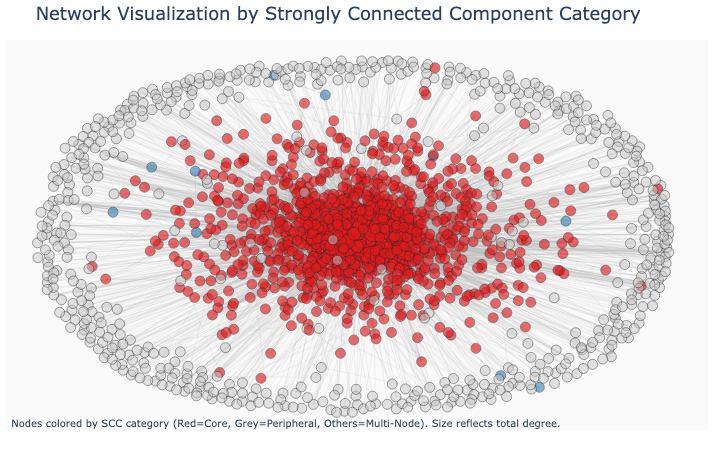
\includegraphics[width=0.9\textwidth]{../scc.png}
    \caption{Network visualization highlighting Strongly Connected Components (SCCs). Nodes could be coloured by SCC category (e.g., Core vs. Periphery) and size reflecting degree.}
    \label{fig:scc_visualization}
\end{figure}

At the local level, the network shows signs of social clustering. The \textbf{unweighted average clustering coefficient} ($\approx 0.0872$) suggests a moderate tendency for users to form triads—higher than random chance. Yet, the \textbf{weighted clustering coefficient} (considering message frequency) drops significantly ($\approx 0.0018$). This disparity implies that while structural triangles exist, they often lack intense, frequent communication loops. Strong, closed triads based on high message volume appear less common than the network's structure might suggest.

\subsection{Identifying Influential Users: Centrality Analysis}
\label{sec:centrality_analysis}

Centrality metrics help identify users holding key positions. We examined several, focusing here on \textbf{Betweenness Centrality}, which identifies network 'brokers'. An approximated weighted calculation highlighted \textbf{User 323} ($\approx 0.118$), \textbf{User 1624} ($\approx 0.086$), and \textbf{User 103} ($\approx 0.086$) as the top intermediaries. These individuals frequently lie on the shortest communication paths, suggesting they bridge different social circles and potentially influence information flow across the network core.

Comparing various centrality measures (including degree, PageRank, and betweenness) via Spearman rank correlations revealed strong positive associations overall. Popularity (in-degree), activity (out-degree), and PageRank influence are highly correlated ($\rho > 0.84$ often), especially between weighted and unweighted versions. This indicates that different facets of importance often coincide. Betweenness centrality, while still strongly correlated ($\rho \approx 0.72 - 0.77$), showed slightly weaker links to degree/PageRank, suggesting its role in capturing brokerage is somewhat distinct. These strong interrelations paint a picture where different forms of network influence are significantly intertwined.

\subsection{Network Patterns: Assortativity and Reciprocity}
\label{sec:degree_patterns}

Examining network-wide connection patterns, we found the network to be \textbf{disassortative}, with a \textbf{degree assortativity coefficient} of approximately \textbf{-0.1375}. This negative value indicates a tendency for high-degree users (hubs) to connect with low-degree users, suggesting a "hub-and-spoke" topology rather than a core of interconnected hubs.

Contrasting this global pattern, interaction directness is high. The \textbf{graph reciprocity} is approximately \textbf{0.6364}, indicating a strong tendency for connections to be mutual; if A messages B, B is highly likely to message A back. This structural tendency towards mutual links is mirrored in individual behavior: a strong positive \textbf{Pearson correlation ($\rho \approx 0.8311$)} exists between user in-degree and out-degree (visualized in Figure \ref{fig:in_out_corr}). Users who receive messages from many people also tend to send them to many. Thus, while the network structure facilitates hub-spoke connections, the interactions themselves show strong mutuality, and active users engage vigorously in both sending and receiving.

\begin{figure}[h!]
    \centering

    \begin{minipage}[b]{0.4\textwidth}
        \centering
        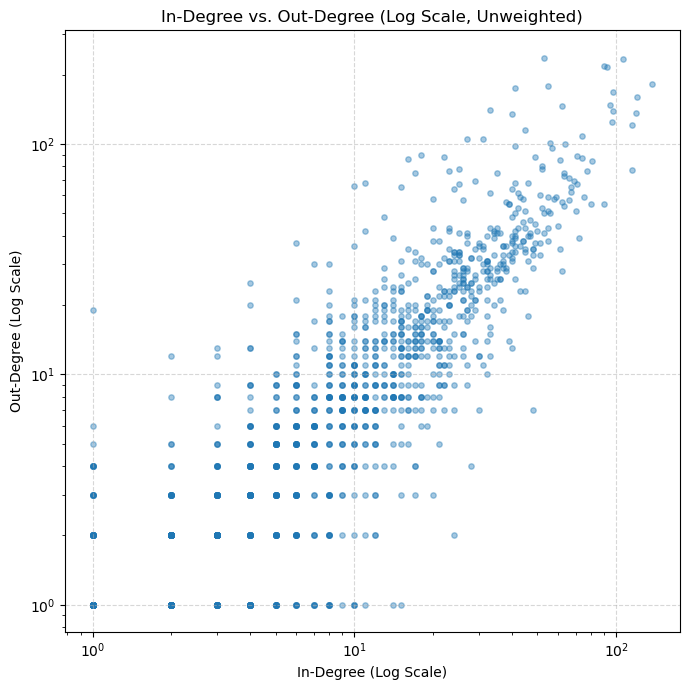
\includegraphics[width=\textwidth]{../inoutdegree.png}
        \caption{Scatter plot of user in-degree vs. out-degree.}
        \label{fig:in_out_corr}
    \end{minipage}
    \hfill
    \begin{minipage}[b]{0.45\textwidth}
        \centering
        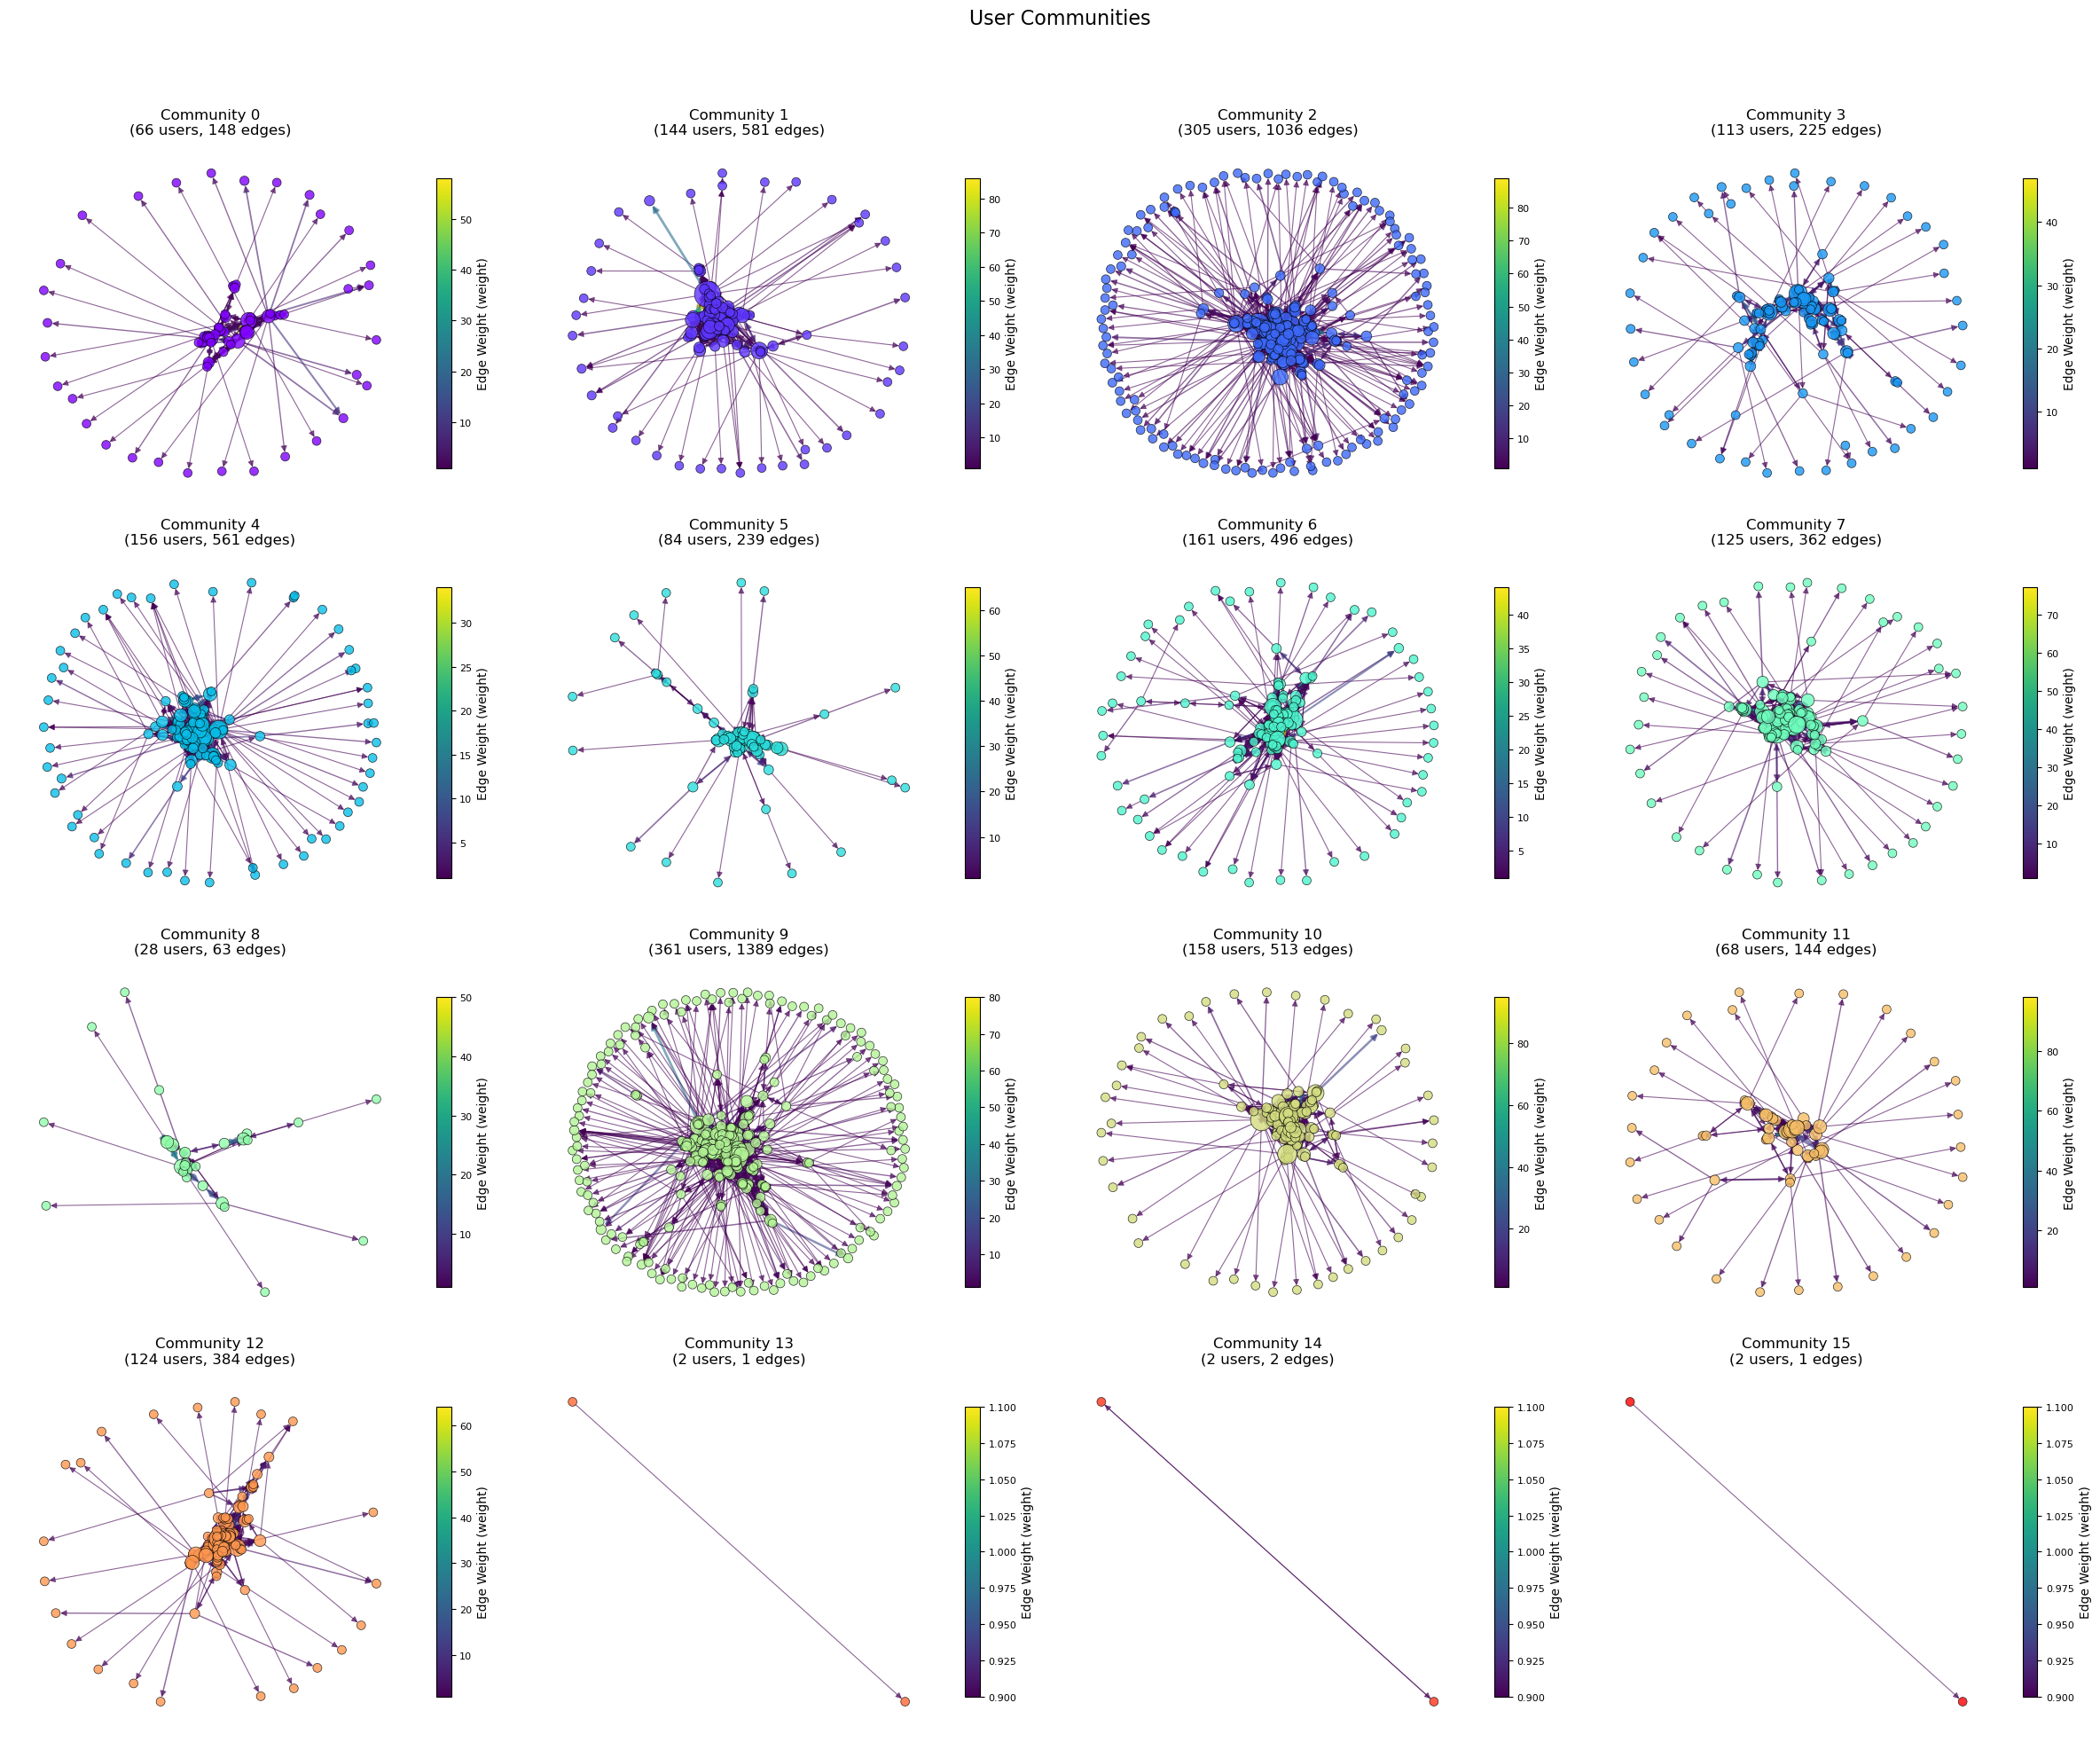
\includegraphics[width=\textwidth]{../communities.png}
        \caption{Network visualization coloured by community membership.}
        \label{fig:community_visualization}
    \end{minipage}

\end{figure}

\subsection{Uncovering Social Groups: Community Structure}
\label{sec:community_structure}

Beyond individual roles, networks often organize into meso-scale communities. Applying the \textbf{Louvain algorithm} directly to the directed graph (using message counts as weights) revealed such underlying organization, partitioning the network into \textbf{16 distinct communities}. The partition achieved a \textbf{modularity} score of approximately \textbf{0.3373}, indicating a meaningful structure where internal connections are significantly denser than expected by chance. This suggests genuine social clustering, visualized in Figure \ref{fig:community_visualization}.


These communities exhibit significant \textbf{heterogeneity in size}. A few large communities (the top five containing \textbf{281, 214, 179, 173, and 162 nodes}) dominate the social landscape, while numerous smaller communities, including pairs, populate the periphery. This suggests a structure with core groups alongside more specialized or isolated clusters.


Analysis of internal characteristics (without detailing per-community stats) reveals further variation. Larger communities tend to be internally sparser (lower density) but contain active members (indicated by higher average internal degrees). Conversely, some smaller communities exhibit higher density, suggesting tighter-knit groups. Importantly, highly central users (in terms of global PageRank or Betweenness) do not appear concentrated within single communities but are distributed across several, potentially serving as bridges between these groups.